% =====================================================================
% University Project Report (LaTeX)
% Title: Quincaillerie Management Web Application
% Student: Farouk BENKHELIFA
% University: ENSTTIC
% Academic Year: 2025/2026
% =====================================================================
\documentclass[12pt,a4paper]{report}

% --- Encoding and typography ---
\usepackage[T1]{fontenc}
\usepackage[utf8]{inputenc}
\usepackage{lmodern}
\usepackage{microtype}

% --- Page layout ---
\usepackage[a4paper,margin=2.5cm]{geometry}
\usepackage{setspace}
\onehalfspacing

% --- Figures, tables, and floats ---
\usepackage{graphicx}
\usepackage{float}
\usepackage{booktabs}
\usepackage{array}
\usepackage{longtable}
\usepackage{caption}
\usepackage{subcaption}

% --- Links and references ---
\usepackage[hidelinks]{hyperref}
\usepackage[nameinlink,noabbrev]{cleveref}

% --- Lists and code ---
\usepackage{enumitem}
\usepackage{listings}
\usepackage{xcolor}

% --- TikZ for diagrams ---
\usepackage{tikz}
\usetikzlibrary{shapes.geometric, arrows.meta, positioning, fit, calc, backgrounds}

% --- Headings ---
\usepackage{titlesec}
\titleformat{\chapter}[hang]{\bfseries\Huge}{\thechapter\,\textbar\,}{0.5em}{}
\titleformat{\section}[hang]{\bfseries\Large}{\thesection}{0.6em}{}

% --- Listing style ---
\definecolor{codebg}{RGB}{248,248,248}
\definecolor{codeframe}{RGB}{220,220,220}
\lstset{
  backgroundcolor=\color{codebg},
  frame=single,
  rulecolor=\color{codeframe},
  basicstyle=\ttfamily\small,
  breaklines=true,
  columns=fullflexible,
  upquote=true
}

% --- Document metadata ---
\newcommand{\ProjectTitle}{Quincaillerie Management Web Application: Inventory and Billing System}
\newcommand{\StudentName}{Farouk BENKHELIFA}
\newcommand{\UniversityName}{ENSTTIC}
\newcommand{\AcademicYear}{2025/2026}

\begin{document}

% =====================================================================
% 1. Page de garde
% =====================================================================
\begin{titlepage}
\centering

\vspace*{1.5cm}

{\Large \UniversityName \par}
\vspace{0.8cm}

{\Large Academic Year: \AcademicYear \par}
\vspace{2.0cm}

{\huge\bfseries \ProjectTitle \par}
\vspace{1.2cm}

{\Large University Project Report \par}
\vspace{2.5cm}

\begin{tabular}{>{\bfseries}p{5.5cm} p{8cm}}
Student name: & \StudentName \\
\end{tabular}

\vfill

% If your university requires additional fields (department, supervisor, jury),
% you can add them here while keeping the requested mandatory items.

\end{titlepage}

\pagenumbering{arabic}
\tableofcontents
\listoffigures

% =====================================================================
% 2. Résumé / Abstract
% =====================================================================
\chapter*{Résumé / Abstract}
\addcontentsline{toc}{chapter}{Résumé / Abstract}

This report presents the design and implementation of a local web application for managing a hardware store (\textit{quincaillerie}). The system supports day-to-day operations such as product catalog management, supplier and category tracking, worker management, invoice (bill) generation, stock movements, and basic analytics through a dashboard. The application was implemented using a modern Laravel backend combined with Inertia.js and a React-based frontend, providing a single-page application (SPA) experience while preserving server-side routing and security patterns.

A central objective of the project is operational reliability in a small-business environment. The solution emphasizes data consistency (especially for stock and billing), usability for non-technical users, and bilingual support (French and Arabic) without altering the layout direction (LTR remains constant to ensure consistent user experience). The project also integrates print-ready invoices and PDF generation.

\textbf{Keywords:} Laravel, Inertia.js, React, Material UI, MySQL, inventory management, billing system, multilingual interface.

% =====================================================================
% 3. Introduction
% =====================================================================
\chapter{Introduction}

\section{Context}
Hardware stores typically manage a diverse inventory (tools, fasteners, safety equipment, electrical materials, etc.) with varying units (pieces, meters, boxes). In such environments, stock visibility and quick billing are essential. Errors in inventory levels can lead to loss of sales (out-of-stock situations), over-ordering, and accounting inconsistencies.

\section{Motivation}
This project was motivated by the practical need for a simple, locally runnable system that streamlines the work of a small store: searching products quickly, issuing invoices, and updating stock automatically. The goal is to reduce time spent on manual bookkeeping, improve accuracy, and provide a professional invoice output suitable for printing.

\section{Problem Statement}
Manual store management approaches (paper notebooks, spreadsheet files, or ad-hoc tools) often suffer from:
\begin{itemize}
  \item inconsistent data formats and duplicated records,
  \item lack of traceability for stock changes,
  \item slow product search and billing,
  \item limited reporting and visibility (low stock, best-selling items),
  \item difficulty maintaining bilingual information.
\end{itemize}

The problem is therefore to design and implement a robust and user-friendly application that supports core operations (products, invoices, stock movements) while ensuring data integrity and enabling bilingual user interaction.

% =====================================================================
% 4. Étude de l’existant
% =====================================================================
\chapter{Étude de l’existant}

\section{Traditional Store Management Problems}
In traditional hardware stores, inventory and invoicing are frequently handled manually or with minimal tooling:
\begin{itemize}
  \item \textbf{Paper-based tracking:} low cost but highly error-prone and difficult to search.
  \item \textbf{Spreadsheets:} more flexible, but typically lack constraints, automated workflows, and proper auditing.
  \item \textbf{Generic POS tools:} may be expensive, require internet connectivity, or do not match local needs (units, bilingual product naming).
\end{itemize}

Common consequences include frequent stock mismatches, difficulty identifying low-stock products in time, and limited ability to analyze sales trends.

\section{Limitations of Manual Systems}
Manual systems rarely guarantee transactional consistency: when an invoice is issued, multiple updates must occur (invoice record, items lines, stock decreases, and optional movement history). Without automation, these steps can be forgotten or performed inconsistently.

Additionally, manual systems do not naturally provide:
\begin{itemize}
  \item unique identifiers and consistent numbering for invoices,
  \item audit trails for inventory changes,
  \item secure access control (roles and authentication),
  \item standardized printable invoices,
  \item multilingual presentation with consistent terminology.
\end{itemize}

% =====================================================================
% 5. Analyse des besoins
% =====================================================================
\chapter{Analyse des besoins}

\section{Stakeholders}
\begin{itemize}
  \item \textbf{Store owner:} supervises inventory, reviews sales, configures store information.
  \item \textbf{Cashier/worker:} searches products, creates invoices, interacts with customers.
  \item \textbf{Administrator:} manages users, settings, and ensures overall system operation.
\end{itemize}

\section{Functional Requirements}
The functional requirements were defined to cover the most frequent operational tasks.

\subsection*{Product Management}
\begin{itemize}
  \item Create, edit, and deactivate products.
  \item Manage product attributes: name (FR/AR), SKU, barcode, unit, purchase/selling price, minimum stock threshold, and optional image.
  \item Search products by name, SKU, or barcode.
  \item Filter and list products by category, supplier, and stock status.
\end{itemize}

\subsection*{Inventory and Stock Movements}
\begin{itemize}
  \item Automatic stock decrease when an invoice is validated.
  \item Stock adjustment operation (add/remove) with reason and traceability.
  \item Visualization of low stock and out-of-stock products.
\end{itemize}

\subsection*{Billing / Invoices}
\begin{itemize}
  \item Create invoices with multiple product lines.
  \item Compute subtotal, global discount, tax, and total.
  \item Print a clean invoice (A4 layout) and export PDF.
  \item Cancel invoices with stock restoration.
  \item Edit invoices when needed (with controlled stock recalculation).
\end{itemize}

\subsection*{Workers and Access}
\begin{itemize}
  \item Manage store workers (cashier, admin, etc.).
  \item Authentication and session protection.
\end{itemize}

\subsection*{Settings and Configuration}
\begin{itemize}
  \item Configure store identity data (store name, owner name, address, phone, tax IDs).
  \item Use these settings on invoices.
\end{itemize}

\subsection*{Multilingual and Theme}
\begin{itemize}
  \item Provide French and Arabic translations for UI labels.
  \item Keep LTR layout regardless of language (translate content only).
  \item Support light and dark mode.
\end{itemize}

\section{Non-Functional Requirements}
\begin{itemize}
  \item \textbf{Usability:} fast product lookup, minimal clicks to create invoices.
  \item \textbf{Reliability:} transactional integrity for billing and stock updates.
  \item \textbf{Security:} authenticated access to all management features.
  \item \textbf{Performance:} acceptable response time for product listing and search in local environment.
  \item \textbf{Maintainability:} clean code structure and separation of concerns.
  \item \textbf{Portability:} local deployment on Windows via Laragon.
\end{itemize}

% =====================================================================
% 6. Choix technologiques
% =====================================================================
\chapter{Choix technologiques}

\section{Laravel}
Laravel is used as the backend framework because it provides:
\begin{itemize}
  \item an expressive MVC architecture,
  \item built-in authentication patterns, routing, validation, and migrations,
  \item strong ecosystem and community documentation,
  \item database abstraction (Eloquent ORM) suitable for rapid development.
\end{itemize}
\textbf{Justification:} For an academic engineering project, Laravel balances productivity and architectural discipline, enabling implementation of robust CRUD operations with consistent conventions.

\section{Inertia.js}
Inertia.js provides SPA-like navigation without building a separate API.
\textbf{Justification:} It reduces complexity by avoiding duplicated routing layers (REST API + SPA router). The server controls routes and authorization while the client renders pages.

\section{React}
React is used for the user interface due to its component model and ecosystem.
\textbf{Justification:} The project benefits from reusable UI components (tables, dialogs, forms), predictable state handling, and strong community support.

\section{Material UI (MUI)}
Material UI accelerates UI development with accessible components.
\textbf{Justification:} It provides consistent design, responsive layout primitives, and advanced widgets (data grids, dialogs) suitable for administrative applications.

\section{MySQL}
MySQL is used as the relational database.
\textbf{Justification:} It is reliable, widely used in industry, and fully supported by Laravel migrations and ORM.

\section{Laragon}
Laragon is used as the local development stack on Windows.
\textbf{Justification:} It simplifies managing Apache/MySQL/PHP and provides a convenient environment for academic demonstrations without cloud deployment.

\section{Vibe Coding (AI-Assisted Development)}
The project was developed using a \textbf{vibe coding} approach, leveraging AI-powered coding assistants (such as GitHub Copilot) to accelerate development. This methodology involves:
\begin{itemize}
  \item describing desired functionality in natural language,
  \item receiving AI-generated code suggestions and implementations,
  \item reviewing, validating, and refining the generated code,
  \item iterating quickly on features with AI guidance.
\end{itemize}
\textbf{Justification:} Vibe coding significantly increased development speed, allowed rapid prototyping, and helped implement best practices by leveraging AI knowledge of modern frameworks and patterns. This approach represents an emerging paradigm in software development that combines human creativity with AI efficiency.

% =====================================================================
% 7. Architecture de l’application
% =====================================================================
\chapter{Architecture de l’application}

\section{Overview}
The application follows a layered architecture:
\begin{itemize}
  \item \textbf{Presentation layer:} React pages and components.
  \item \textbf{Application layer:} Laravel controllers and queries, coordinating use cases.
  \item \textbf{Domain/data layer:} Eloquent models, migrations, and database.
\end{itemize}

\section{Backend Architecture}
The backend uses Laravel's MVC structure:
\begin{itemize}
  \item \textbf{Controllers} handle HTTP requests, validation, and orchestration.
  \item \textbf{Models} represent entities such as Product, Bill, BillItem, Worker, Category, Supplier.
  \item \textbf{Migrations} define database schema versioning.
  \item \textbf{Services/Domain logic} is encapsulated in model methods (e.g., stock adjustment) and query classes.
\end{itemize}

\section{Frontend Architecture}
The frontend is composed of:
\begin{itemize}
  \item \textbf{Inertia pages:} each page corresponds to a server route (Dashboard, Products, Bills, Settings, etc.).
  \item \textbf{Reusable components:} product table, confirmation dialogs, printable invoice component.
  \item \textbf{Context providers:} language and theme preferences.
\end{itemize}

\section{Database Architecture}
The database uses normalized tables:
\begin{itemize}
  \item product catalog tables (products, categories, suppliers),
  \item billing tables (bills, bill\_items),
  \item inventory audit (inventory\_movements),
  \item configuration (settings),
  \item authentication/session tables.
\end{itemize}

\section{MVC + Inertia Explanation}
In a classic SPA, the frontend consumes an API. With Inertia:
\begin{itemize}
  \item The server defines routes and performs authorization.
  \item The server returns an Inertia response containing props (data).
  \item The React client renders the page component for that route.
\end{itemize}
This model keeps the security and routing logic on the server while preserving smooth client navigation.

% =====================================================================
% 8. Modélisation
% =====================================================================
\chapter{Modélisation}

\section{UML Diagrams (Description)}
The following diagrams are recommended for a complete academic submission. They should be produced using tools such as StarUML, Visual Paradigm, or diagrams.net, then exported as PNG/PDF for insertion.

\subsection{Use Case Diagram}
It should include actors (Admin, Cashier/Worker, Owner) and use cases such as: manage products, create invoice, cancel invoice, adjust stock, manage workers, update settings.

% ---------------------------------------------------------------------
% INSERTION GUIDE (DIAGRAMS)
% ---------------------------------------------------------------------
% How to add an image:
% 1) Create a folder named "figures" next to this .tex file.
% 2) Export your diagram as PNG (e.g., figures/usecase.png).
% 3) Replace the placeholder box below with \includegraphics.
% Example:
%   \includegraphics[width=0.95\textwidth]{figures/usecase.png}
% ---------------------------------------------------------------------

% --- UML Use Case Diagram (TikZ) ---
\begin{figure}[H]
\centering
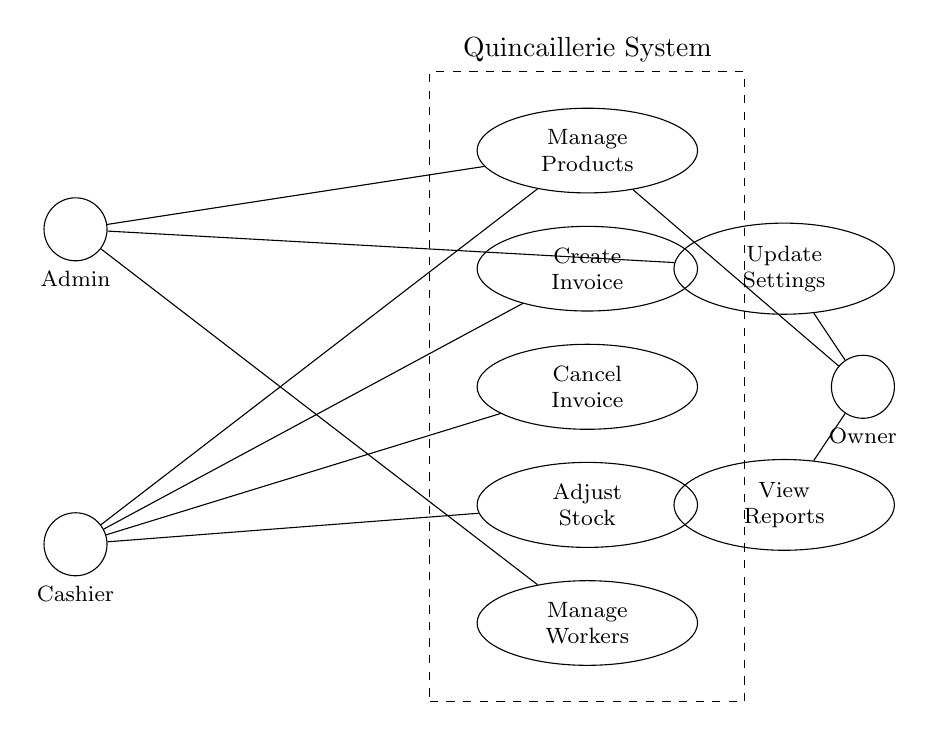
\begin{tikzpicture}[
    actor/.style={circle, draw, minimum size=0.8cm, font=\footnotesize},
    usecase/.style={ellipse, draw, minimum width=2.8cm, minimum height=1cm, align=center, font=\footnotesize},
    system/.style={rectangle, draw, dashed, inner sep=0.5cm}
]
% Actors
\node[actor, label=below:{\footnotesize Admin}] (admin) at (-5, 0) {};
\node[actor, label=below:{\footnotesize Cashier}] (cashier) at (-5, -4) {};
\node[actor, label=below:{\footnotesize Owner}] (owner) at (5, -2) {};

% System boundary
\begin{scope}[on background layer]
\node[system, fit={(0,-5.5) (3,1.5)}, label=above:{Quincaillerie System}] (sys) {};
\end{scope}

% Use cases
\node[usecase] (uc1) at (1.5, 1) {Manage\\Products};
\node[usecase] (uc2) at (1.5, -0.5) {Create\\Invoice};
\node[usecase] (uc3) at (1.5, -2) {Cancel\\Invoice};
\node[usecase] (uc4) at (1.5, -3.5) {Adjust\\Stock};
\node[usecase] (uc5) at (1.5, -5) {Manage\\Workers};
\node[usecase] (uc6) at (4, -0.5) {Update\\Settings};
\node[usecase] (uc7) at (4, -3.5) {View\\Reports};

% Connections
\draw (admin) -- (uc1);
\draw (admin) -- (uc5);
\draw (admin) -- (uc6);
\draw (cashier) -- (uc2);
\draw (cashier) -- (uc3);
\draw (cashier) -- (uc4);
\draw (cashier) -- (uc1);
\draw (owner) -- (uc6);
\draw (owner) -- (uc7);
\draw (owner) -- (uc1);

\end{tikzpicture}
\caption{UML Use Case Diagram.}
\label{fig:uml-usecase}
\end{figure}

\subsection{Class Diagram}
A class diagram should represent core entities and relations, for example:
\begin{itemize}
  \item Product linked to Category and Suppliers.
  \item Bill linked to BillItem lines.
  \item InventoryMovement linked to Product and optionally to Bill.
\end{itemize}

\begin{figure}[H]
\centering
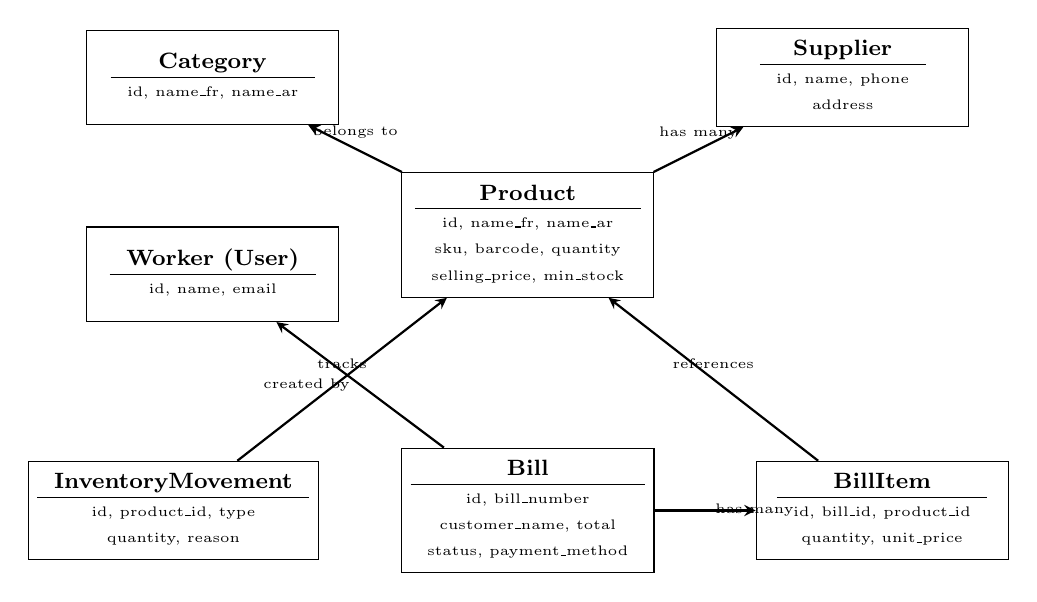
\begin{tikzpicture}[
    class/.style={rectangle, draw, minimum width=3.2cm, minimum height=1.2cm, font=\footnotesize},
    classname/.style={font=\footnotesize\bfseries},
    attr/.style={font=\tiny, align=left},
    relation/.style={->, >=stealth, thick}
]

% Classes
\node[class] (product) at (0, 0) {
    \begin{tabular}{c}
    \textbf{Product} \\ \hline
    {\tiny id, name\_fr, name\_ar} \\
    {\tiny sku, barcode, quantity} \\
    {\tiny selling\_price, min\_stock}
    \end{tabular}
};

\node[class] (category) at (-4, 2) {
    \begin{tabular}{c}
    \textbf{Category} \\ \hline
    {\tiny id, name\_fr, name\_ar}
    \end{tabular}
};

\node[class] (supplier) at (4, 2) {
    \begin{tabular}{c}
    \textbf{Supplier} \\ \hline
    {\tiny id, name, phone} \\
    {\tiny address}
    \end{tabular}
};

\node[class] (bill) at (0, -3.5) {
    \begin{tabular}{c}
    \textbf{Bill} \\ \hline
    {\tiny id, bill\_number} \\
    {\tiny customer\_name, total} \\
    {\tiny status, payment\_method}
    \end{tabular}
};

\node[class] (billitem) at (4.5, -3.5) {
    \begin{tabular}{c}
    \textbf{BillItem} \\ \hline
    {\tiny id, bill\_id, product\_id} \\
    {\tiny quantity, unit\_price}
    \end{tabular}
};

\node[class] (movement) at (-4.5, -3.5) {
    \begin{tabular}{c}
    \textbf{InventoryMovement} \\ \hline
    {\tiny id, product\_id, type} \\
    {\tiny quantity, reason}
    \end{tabular}
};

\node[class] (worker) at (-4, -0.5) {
    \begin{tabular}{c}
    \textbf{Worker (User)} \\ \hline
    {\tiny id, name, email}
    \end{tabular}
};

% Relations
\draw[relation] (product) -- node[above, font=\tiny] {belongs to} (category);
\draw[relation] (product) -- node[above, font=\tiny] {has many} (supplier);
\draw[relation] (bill) -- node[right, font=\tiny] {has many} (billitem);
\draw[relation] (billitem) -- node[above, font=\tiny] {references} (product);
\draw[relation] (movement) -- node[above, font=\tiny] {tracks} (product);
\draw[relation] (bill) -- node[left, font=\tiny] {created by} (worker);

\end{tikzpicture}
\caption{UML Class Diagram showing core entities and relationships.}
\label{fig:uml-class}
\end{figure}

\subsection{Sequence Diagram (Invoice Creation)}
A sequence diagram can clarify the transactional workflow:
\begin{enumerate}
  \item User selects products and confirms invoice.
  \item Client sends request to server.
  \item Server validates data and begins transaction.
  \item For each item: check stock, create bill item, decrease stock, record movement.
  \item Commit transaction and return success response.
\end{enumerate}

\begin{figure}[H]
\centering
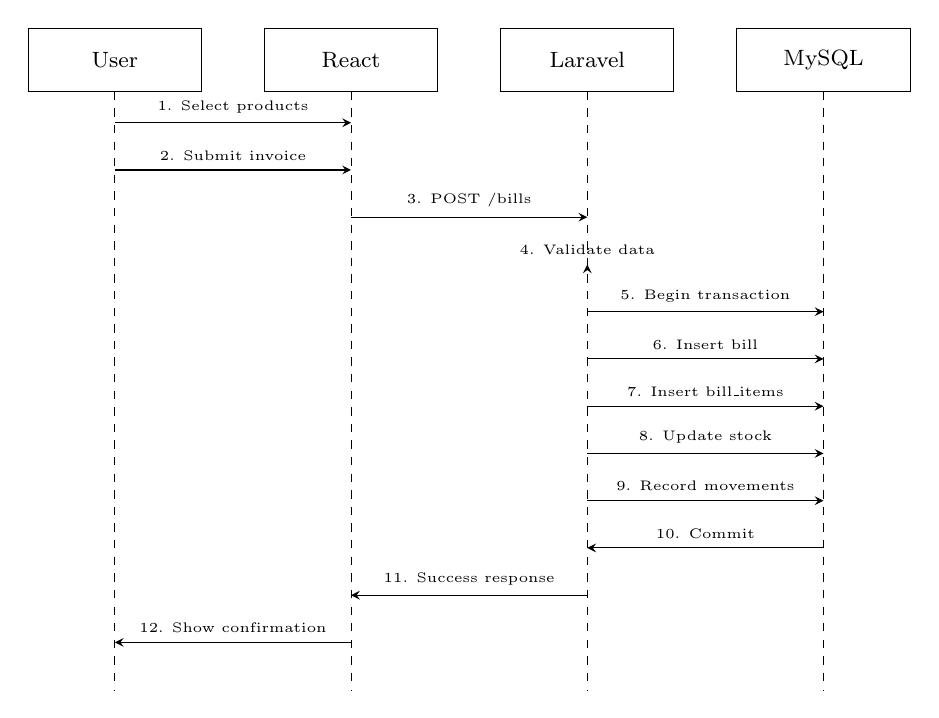
\begin{tikzpicture}[
    object/.style={rectangle, draw, minimum width=2.2cm, minimum height=0.8cm, font=\footnotesize},
    lifeline/.style={dashed},
    arrow/.style={->, >=stealth},
    note/.style={font=\tiny}
]

% Objects
\node[object] (user) at (0, 0) {User};
\node[object] (react) at (3, 0) {React};
\node[object] (laravel) at (6, 0) {Laravel};
\node[object] (db) at (9, 0) {MySQL};

% Lifelines
\draw[lifeline] (user) -- (0, -8);
\draw[lifeline] (react) -- (3, -8);
\draw[lifeline] (laravel) -- (6, -8);
\draw[lifeline] (db) -- (9, -8);

% Messages
\draw[arrow] (0, -0.8) -- node[above, note] {1. Select products} (3, -0.8);
\draw[arrow] (0, -1.4) -- node[above, note] {2. Submit invoice} (3, -1.4);
\draw[arrow] (3, -2) -- node[above, note] {3. POST /bills} (6, -2);
\draw[arrow] (6, -2.6) -- node[above, note] {4. Validate data} (6, -2.6);
\draw[arrow] (6, -3.2) -- node[above, note] {5. Begin transaction} (9, -3.2);
\draw[arrow] (6, -3.8) -- node[above, note] {6. Insert bill} (9, -3.8);
\draw[arrow] (6, -4.4) -- node[above, note] {7. Insert bill\_items} (9, -4.4);
\draw[arrow] (6, -5) -- node[above, note] {8. Update stock} (9, -5);
\draw[arrow] (6, -5.6) -- node[above, note] {9. Record movements} (9, -5.6);
\draw[arrow] (9, -6.2) -- node[above, note] {10. Commit} (6, -6.2);
\draw[arrow] (6, -6.8) -- node[above, note] {11. Success response} (3, -6.8);
\draw[arrow] (3, -7.4) -- node[above, note] {12. Show confirmation} (0, -7.4);

\end{tikzpicture}
\caption{Sequence Diagram for invoice creation workflow.}
\label{fig:uml-seq}
\end{figure}

\section{Database Schema Explanation}
The relational schema is designed to ensure consistency between invoices and inventory.

\subsection{Core Tables}
\begin{itemize}
  \item \textbf{products:} stores product identity, pricing, unit, current quantity, and optional image path.
  \item \textbf{categories:} classifies products.
  \item \textbf{suppliers:} stores supplier information.
  \item \textbf{product\_supplier:} many-to-many relationship with pivot metadata.
\end{itemize}

\subsection{Billing Tables}
\begin{itemize}
  \item \textbf{bills:} stores invoice header information (number, customer info, totals, payment method, status).
  \item \textbf{bill\_items:} line items for each product in a bill.
\end{itemize}

\subsection{Inventory Audit Table}
\begin{itemize}
  \item \textbf{inventory\_movements:} logs stock changes (purchase, sale, adjustment, return), enabling traceability.
\end{itemize}

\begin{figure}[H]
\centering
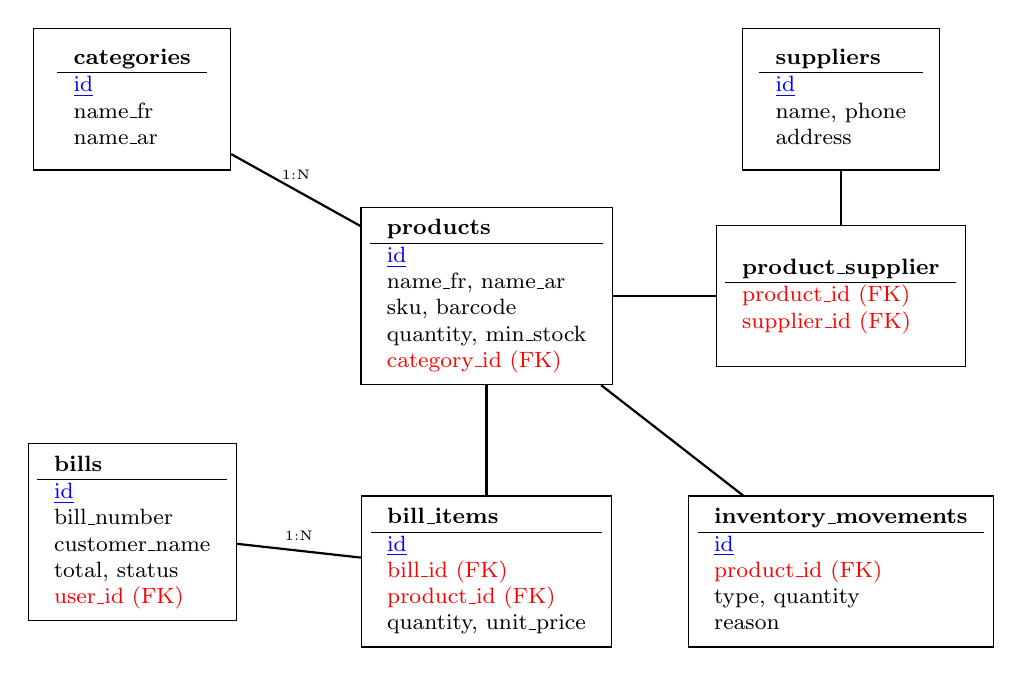
\begin{tikzpicture}[
    entity/.style={rectangle, draw, minimum width=2.5cm, minimum height=1.8cm, font=\footnotesize},
    attr/.style={font=\tiny},
    pk/.style={font=\tiny, text=blue},
    fk/.style={font=\tiny, text=red},
    relation/.style={thick}
]

% Entities
\node[entity] (products) at (0, 0) {
    \begin{tabular}{l}
    \textbf{products} \\ \hline
    \textcolor{blue}{\underline{id}} \\
    name\_fr, name\_ar \\
    sku, barcode \\
    quantity, min\_stock \\
    \textcolor{red}{category\_id (FK)}
    \end{tabular}
};

\node[entity] (categories) at (-4.5, 2.5) {
    \begin{tabular}{l}
    \textbf{categories} \\ \hline
    \textcolor{blue}{\underline{id}} \\
    name\_fr \\
    name\_ar
    \end{tabular}
};

\node[entity] (suppliers) at (4.5, 2.5) {
    \begin{tabular}{l}
    \textbf{suppliers} \\ \hline
    \textcolor{blue}{\underline{id}} \\
    name, phone \\
    address
    \end{tabular}
};

\node[entity] (prodsup) at (4.5, 0) {
    \begin{tabular}{l}
    \textbf{product\_supplier} \\ \hline
    \textcolor{red}{product\_id (FK)} \\
    \textcolor{red}{supplier\_id (FK)}
    \end{tabular}
};

\node[entity] (bills) at (-4.5, -3) {
    \begin{tabular}{l}
    \textbf{bills} \\ \hline
    \textcolor{blue}{\underline{id}} \\
    bill\_number \\
    customer\_name \\
    total, status \\
    \textcolor{red}{user\_id (FK)}
    \end{tabular}
};

\node[entity] (billitems) at (0, -3.5) {
    \begin{tabular}{l}
    \textbf{bill\_items} \\ \hline
    \textcolor{blue}{\underline{id}} \\
    \textcolor{red}{bill\_id (FK)} \\
    \textcolor{red}{product\_id (FK)} \\
    quantity, unit\_price
    \end{tabular}
};

\node[entity] (movements) at (4.5, -3.5) {
    \begin{tabular}{l}
    \textbf{inventory\_movements} \\ \hline
    \textcolor{blue}{\underline{id}} \\
    \textcolor{red}{product\_id (FK)} \\
    type, quantity \\
    reason
    \end{tabular}
};

% Relations
\draw[relation] (categories) -- node[above, font=\tiny] {1:N} (products);
\draw[relation] (products) -- (prodsup);
\draw[relation] (suppliers) -- (prodsup);
\draw[relation] (bills) -- node[above, font=\tiny] {1:N} (billitems);
\draw[relation] (products) -- (billitems);
\draw[relation] (products) -- (movements);

\end{tikzpicture}
\caption{Entity-Relationship Diagram of the database schema.}
\label{fig:db-er}
\end{figure}

% =====================================================================
% 9. Fonctionnalités principales
% =====================================================================
\chapter{Fonctionnalités principales}

\section{Products Management}
The products module supports the full life cycle:
\begin{itemize}
  \item creation of products with essential identifiers (SKU, barcode),
  \item assignment to categories and suppliers,
  \item image upload (optional) for easier recognition,
  \item fast search and listing with pagination,
  \item low-stock indication based on threshold.
\end{itemize}

\section{Workers}
Workers represent store staff. The system enables:
\begin{itemize}
  \item adding and updating worker profiles,
  \item assigning invoices to workers for traceability.
\end{itemize}

\section{Bills / Invoices}
The billing module provides:
\begin{itemize}
  \item multi-item invoice creation,
  \item automatic totals calculation (subtotal, discount, tax, total),
  \item invoice cancellation with stock restoration,
  \item invoice editing with controlled recalculation of stock,
  \item PDF export and print-ready invoice view.
\end{itemize}

\section{Inventory}
Inventory operations include:
\begin{itemize}
  \item stock adjustments (increase/decrease),
  \item automatic stock decreases on sales,
  \item audit trail of movements with reasons and timestamps.
\end{itemize}

\section{Multilingual Support (French / Arabic)}
The interface supports French and Arabic translations for most labels. A key design decision is to keep the layout direction in LTR to avoid UI instability; only the language of labels and content changes.

\section{Light \& Dark Mode}
Theme toggling improves usability across lighting conditions. The design relies on a consistent component library to ensure readability and contrast in both modes.

% =====================================================================
% 10. Interface utilisateur
% =====================================================================
\chapter{Interface utilisateur}

\section{UX Principles}
The UI was designed according to practical constraints of a store environment:
\begin{itemize}
  \item \textbf{Speed:} minimize navigation steps for frequent tasks.
  \item \textbf{Clarity:} consistent forms and tables, readable typography.
  \item \textbf{Feedback:} confirmation dialogs and toast notifications for actions.
\end{itemize}

\section{Ease of Use}
Key choices that improve ease of use include:
\begin{itemize}
  \item product search with suggestions,
  \item multi-selection when adding items to a bill,
  \item integer quantity input for faster cash desk operations,
  \item printable invoice preview before printing.
\end{itemize}

\section{Accessibility}
Material UI components support accessibility considerations:
\begin{itemize}
  \item keyboard navigation for form elements,
  \item consistent focus management in dialogs,
  \item sufficient contrast in theme modes.
\end{itemize}

% ---------------------------------------------------------------------
% SCREENSHOTS
% ---------------------------------------------------------------------

\begin{figure}[H]
\centering
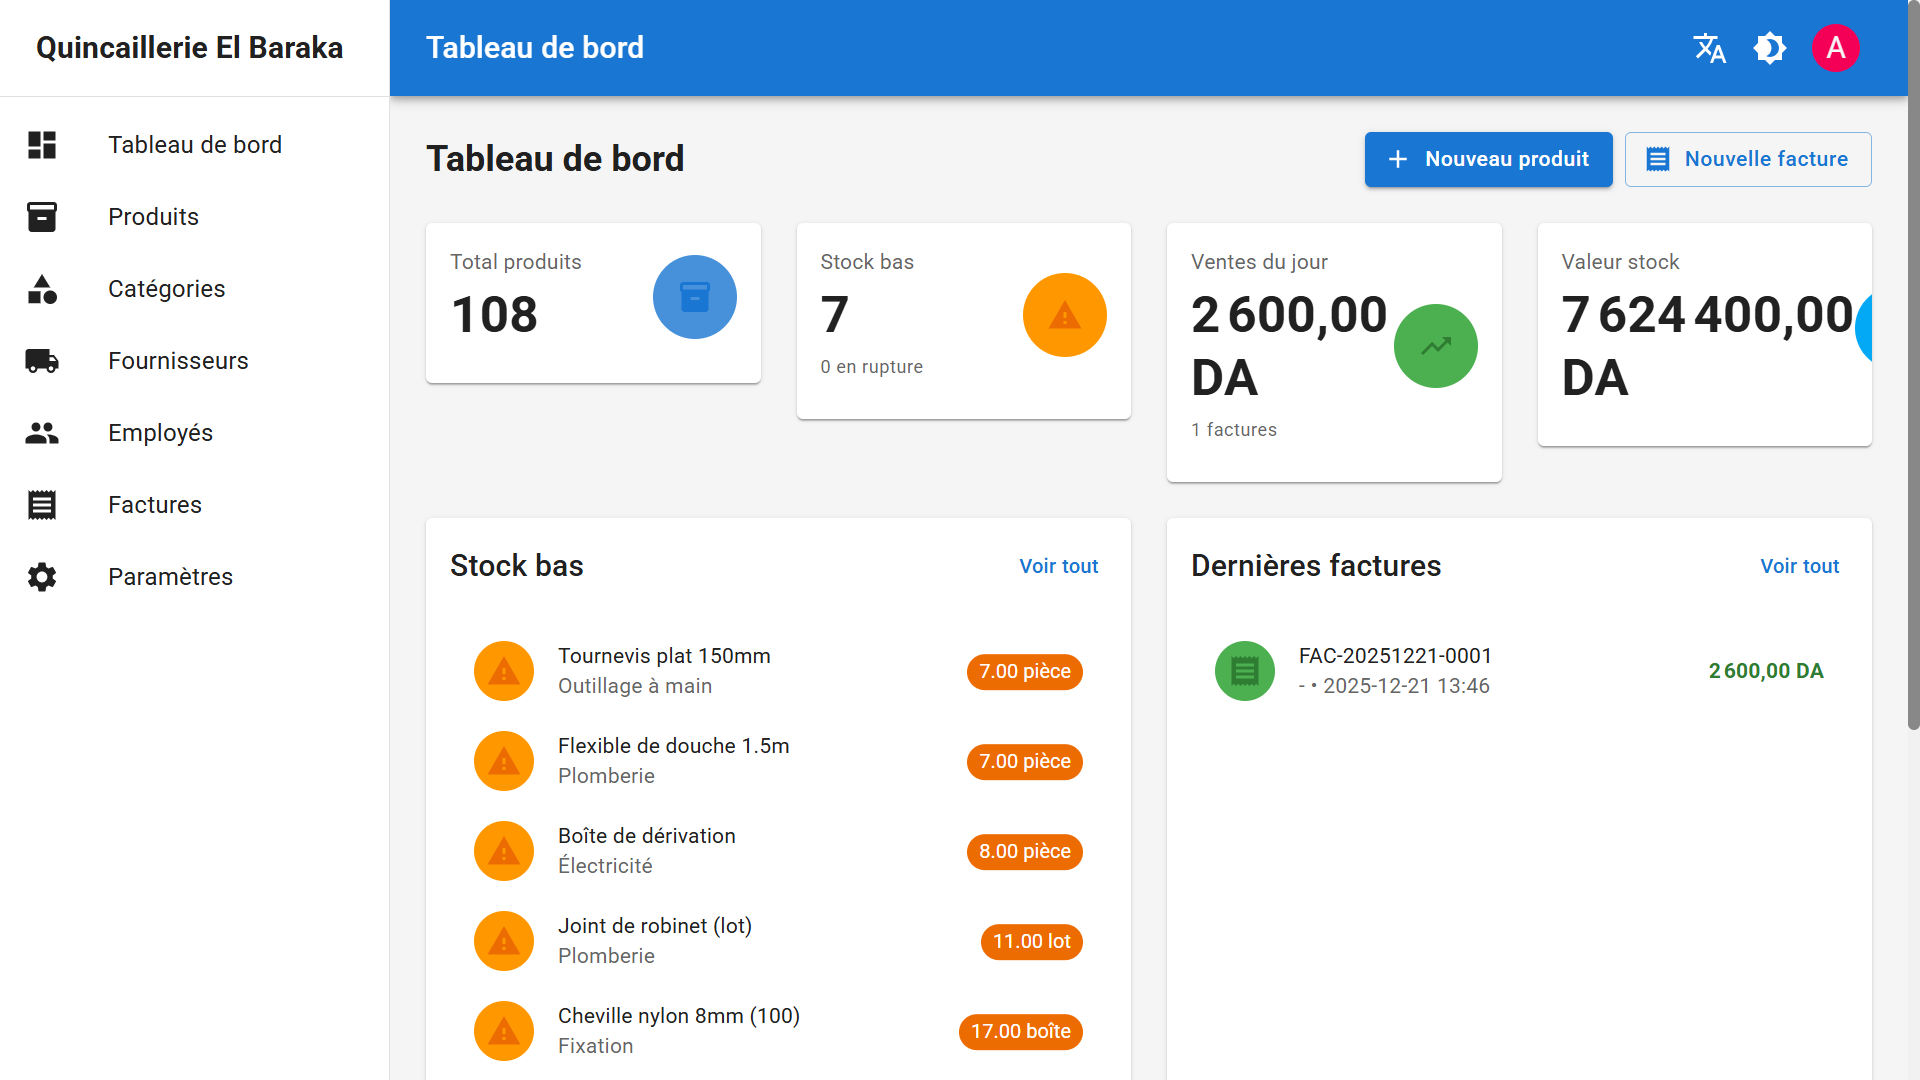
\includegraphics[width=0.95\textwidth]{figures/dashboard.png}
\caption{Dashboard showing key statistics: total products, low stock alerts, daily sales, and stock value. The interface displays recent invoices and products requiring attention.}
\label{fig:ui-dashboard}
\end{figure}

\begin{figure}[H]
\centering
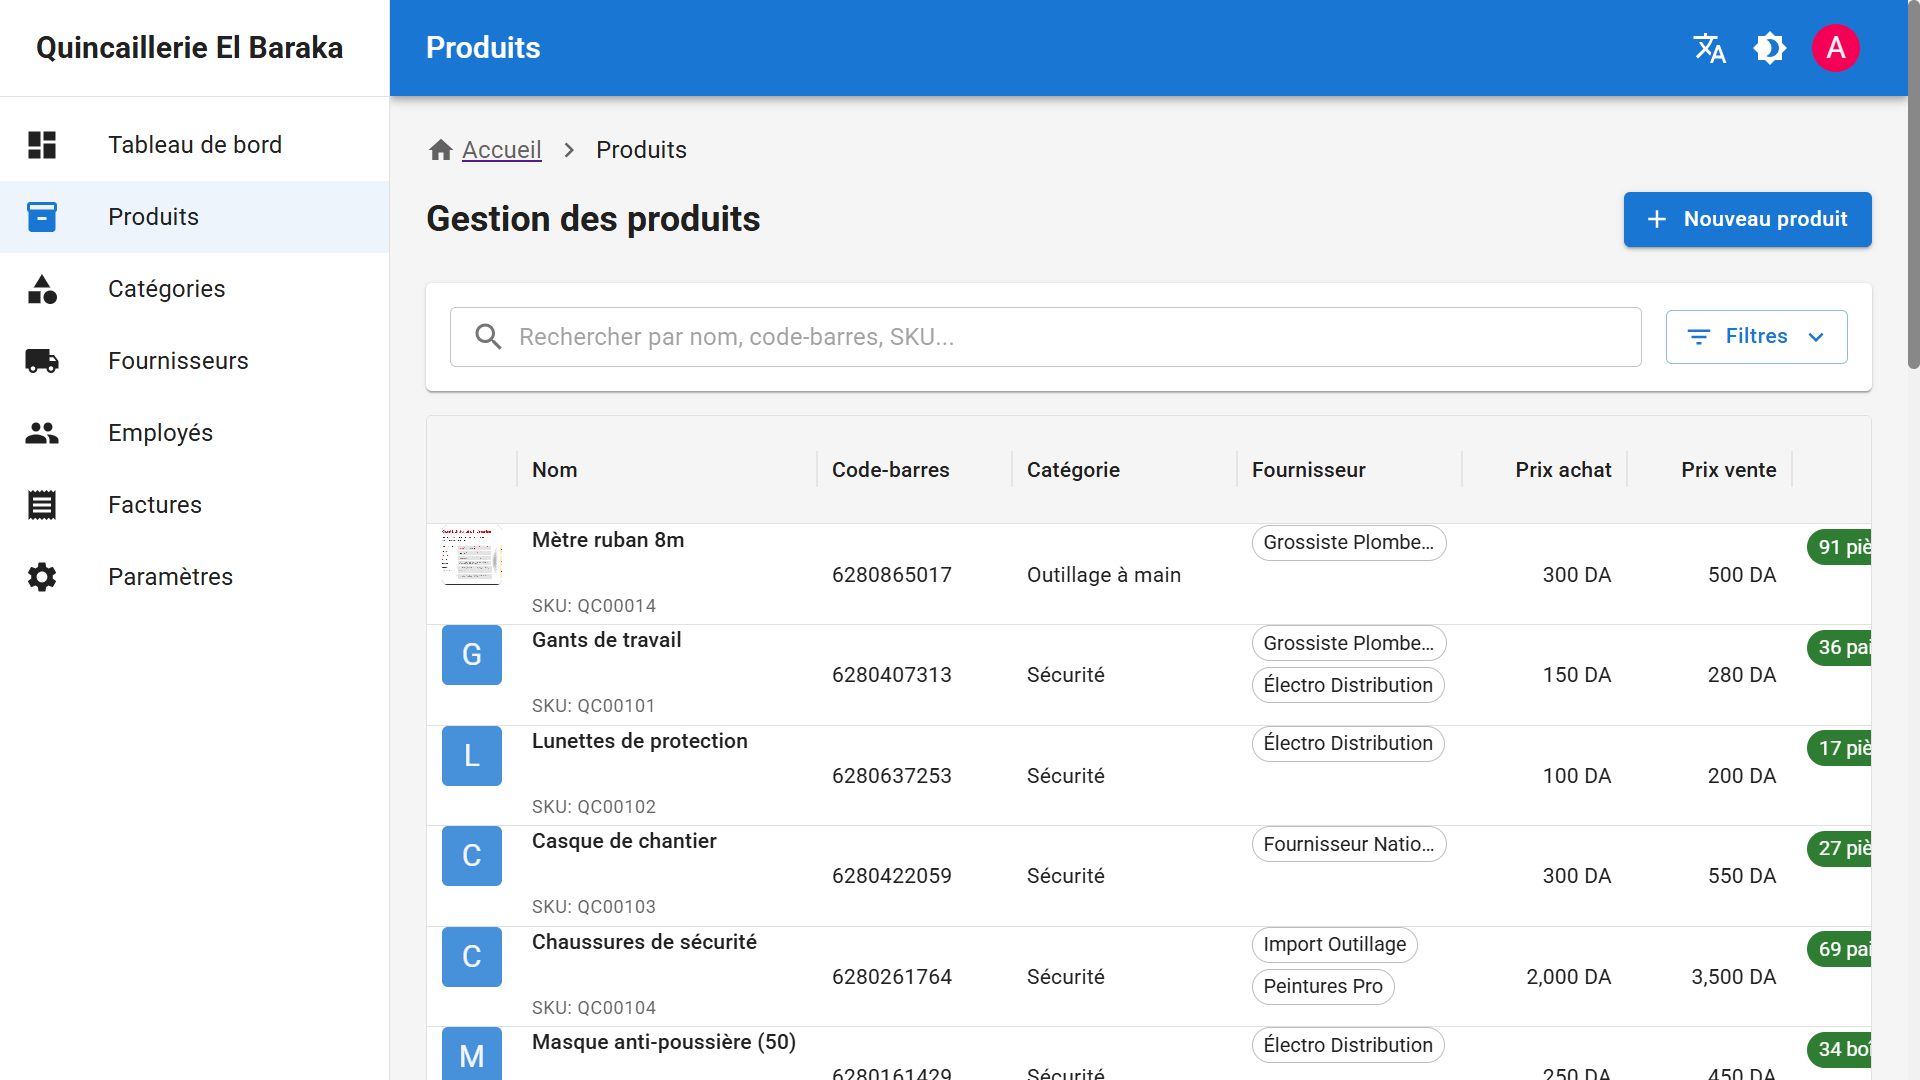
\includegraphics[width=0.95\textwidth]{figures/products-list.png}
\caption{Products list with search functionality, barcode display, category and supplier information, purchase and selling prices, and stock quantities.}
\label{fig:ui-products}
\end{figure}

\begin{figure}[H]
\centering
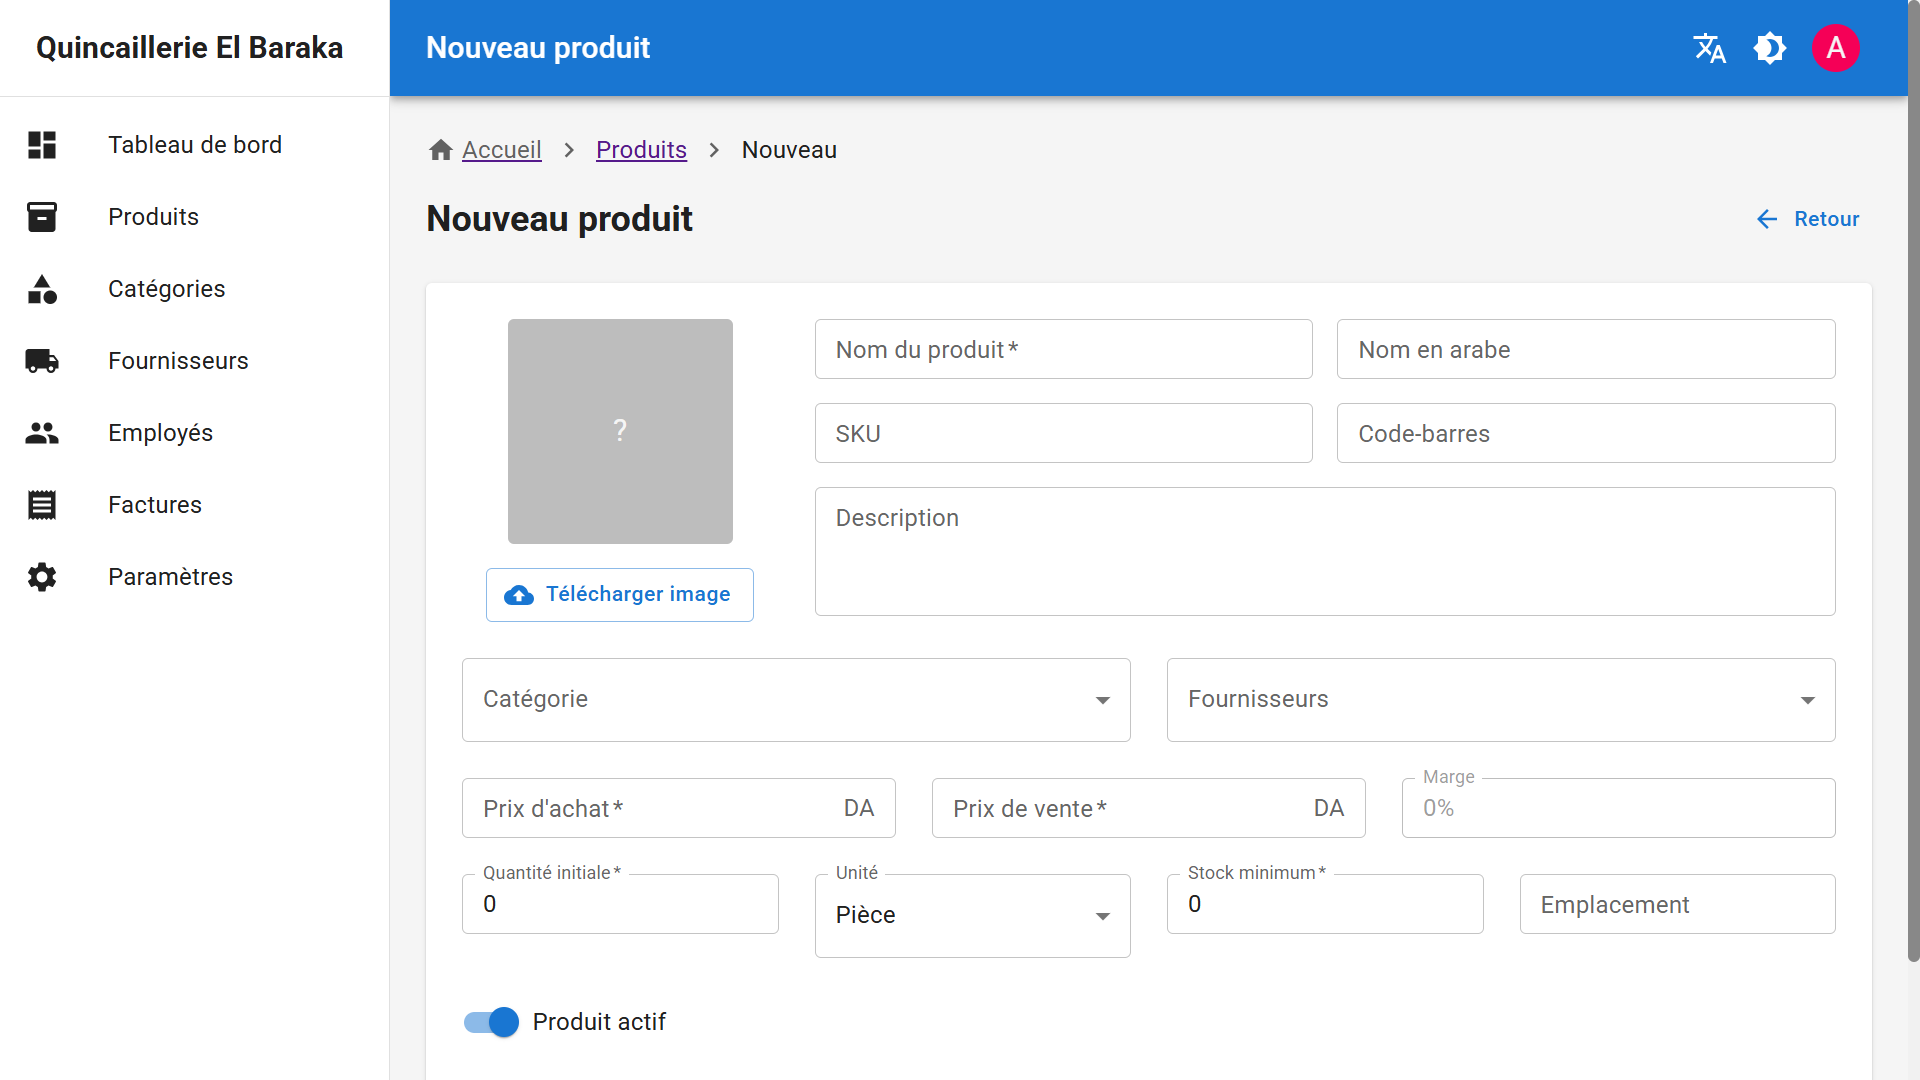
\includegraphics[width=0.95\textwidth]{figures/product-create.png}
\caption{Product creation form with bilingual name fields (French/Arabic), SKU, barcode, category and supplier selection, pricing, quantity, and unit configuration.}
\label{fig:ui-product-create}
\end{figure}

\begin{figure}[H]
\centering
\includegraphics[width=0.95\textwidth]{figures/bill-print.png}
\caption{Invoice print preview with PDF export option. The invoice displays store information, customer details, itemized products, and totals with amount in words.}
\label{fig:ui-bill-print}
\end{figure}

% =====================================================================
% 11. Tests et validation
% =====================================================================
\chapter{Tests et validation}

\section{Testing Strategy}
Testing and validation were performed at multiple levels:
\begin{itemize}
  \item \textbf{Functional testing:} verifying each module (products, bills, settings) through user flows.
  \item \textbf{Validation rules testing:} ensuring backend validation rejects invalid inputs (negative prices, empty invoice items).
  \item \textbf{Transactional testing:} verifying stock consistency after invoice creation, cancellation, and editing.
  \item \textbf{UI testing:} verifying responsive behavior, theme switching, and language switching.
\end{itemize}

\section{Key Validation Scenarios}
\subsection*{Invoice Creation}
\begin{itemize}
  \item Create an invoice with multiple items, verify totals and correct stock decrease.
  \item Attempt to create an invoice with insufficient stock, verify request is rejected.
\end{itemize}

\subsection*{Invoice Cancellation}
\begin{itemize}
  \item Cancel an invoice, verify stock restoration and invoice status update.
\end{itemize}

\subsection*{Invoice Editing}
\begin{itemize}
  \item Modify quantities and items, verify stock is restored then recalculated.
  \item Ensure cancelled invoices cannot be edited (business rule).
\end{itemize}

\subsection*{Settings Update}
\begin{itemize}
  \item Update store information, verify it appears on invoices and persists in database.
\end{itemize}

\section{Print and PDF Validation}
\begin{itemize}
  \item Print preview generates clean invoice layout without UI controls.
  \item PDF export produces consistent A4 formatting.
\end{itemize}

% =====================================================================
% 12. Conclusion et perspectives
% =====================================================================
\chapter{Conclusion et perspectives}

\section{Conclusion}
This project demonstrates the implementation of a complete local management system for a hardware store, covering products, billing, and inventory tracking with bilingual support. The application integrates modern web technologies while maintaining a clear separation of concerns via Laravel MVC and Inertia-driven pages.

\section{Future Improvements}
Potential improvements include:
\begin{itemize}
  \item role-based authorization policies for fine-grained access control,
  \item advanced reporting (sales by category, profit analytics),
  \item barcode scanner optimization for faster checkout,
  \item backup/export features (CSV export, database backup workflow),
  \item deployment packaging for offline distribution (prebuilt assets, installer).
\end{itemize}

\end{document}
